\question
Близится к концу строительство боевой станции "Звезда Смерти", и сам Император Палпатин приехал оценить сооружение. К сожалению, он остался очень недоволен решениями ведущих инженеров проекта по расположению коридоров, и призвал вас, опытнейшего специалиста, занять место ваших таинственно пропавших предшественников. 

Вам предоставляется граф – схема строения станции. Вершины — важные узлы, рёбра — пути, соединяющие их. От вас требуется дополнить граф так, чтобы число компонент рёберной двусвязности было минимальным. Необходимым требованием удобства перемещения по станции также является Гамильтоновость полученного графа. 

При этом не забывайте, что даже Имперские ресурсы ограничены, поэтому вам запрещается добавлять новые вершины в граф, а рёбер нужно использовать как можно меньше. После преобразования посчитайте и укажите количество компонент рёберной двусвязности.

\begin{minipage}[h]{0.45\linewidth}
\center{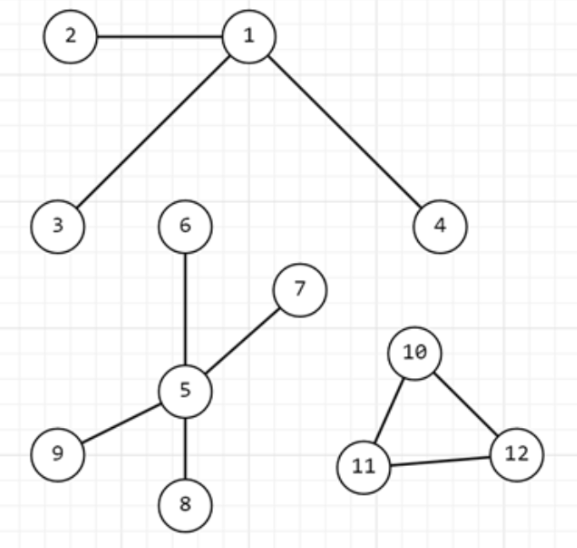
\includegraphics[width=0.7\textwidth]{pic/44.png} }
\end{minipage}

---------------

Автор -- Александр Гущенко
